\subsection{Progettazione di Dettagglio e Codifica}
\label{progettazione_di_dettaglio}
\textbf{Periodo:} dal 2020-03-09 al 2020-04-02 

La fase inizia appena concluca la precedente e termina con la \textit{Revisione di Qualifica}. 

Le precondizioni sono:
\begin{itemize}
    \item Le postcondizioni della fase precedente sono state soddisfatte.
\end{itemize}

Le postcondizioni sono:
\begin{itemize}
    \item Aggiornamento e correzione dei documenti già prodotti;
    \item Realizzazione dei diagrammi delle classi e delle attività;
    \item Completamento codifica e relativa verifica;
    \item Redazione manuale utente e manuale sviluppatore;
    \item Consegna dei documenti richiesti in entrata alla \textit{Revisione di Qualifica};
    \item Ultimata preparazione della presentazione da esporre in sede di revisione.
\end{itemize}

È composta da sei incrementi e nuove attività:

\begin{itemize}
    \item \textbf{Incremento e Verifica:} i documenti già prodotti vengono migliorati e aggiornati se necessario (\textit{\NdP}, \textit{\PdP}, \textit{Glossario},\textit{\PdQ}, \textit{\AdR}, \textit{Technology Baseline}); 
    \item \textbf{Product Baseline:} Segue la \textit{Technology Baseline}; vengono studiati meglio design pattern, classi e attività necessari alla codifica;
    \item \textbf{Specifica Tecnica:} Viene realizzato un documento contenente tute le caratteristiche del prodotto e le motivazione che hanno portato alla loro scelta;
    \item \textbf{Codifica:} Viene scritto il codice con relativa verifica;
    \item \textbf{Manuale Utente:} Viene redatto un documento che rappresenta delle istruzione d'uso specifico per l'utente.
\end{itemize}

\newpage
\subsubsection{Diagramma di Gantt: Progettazione di Dettaglio e Codifica}
\begin{figure}[ht]
    \centering
    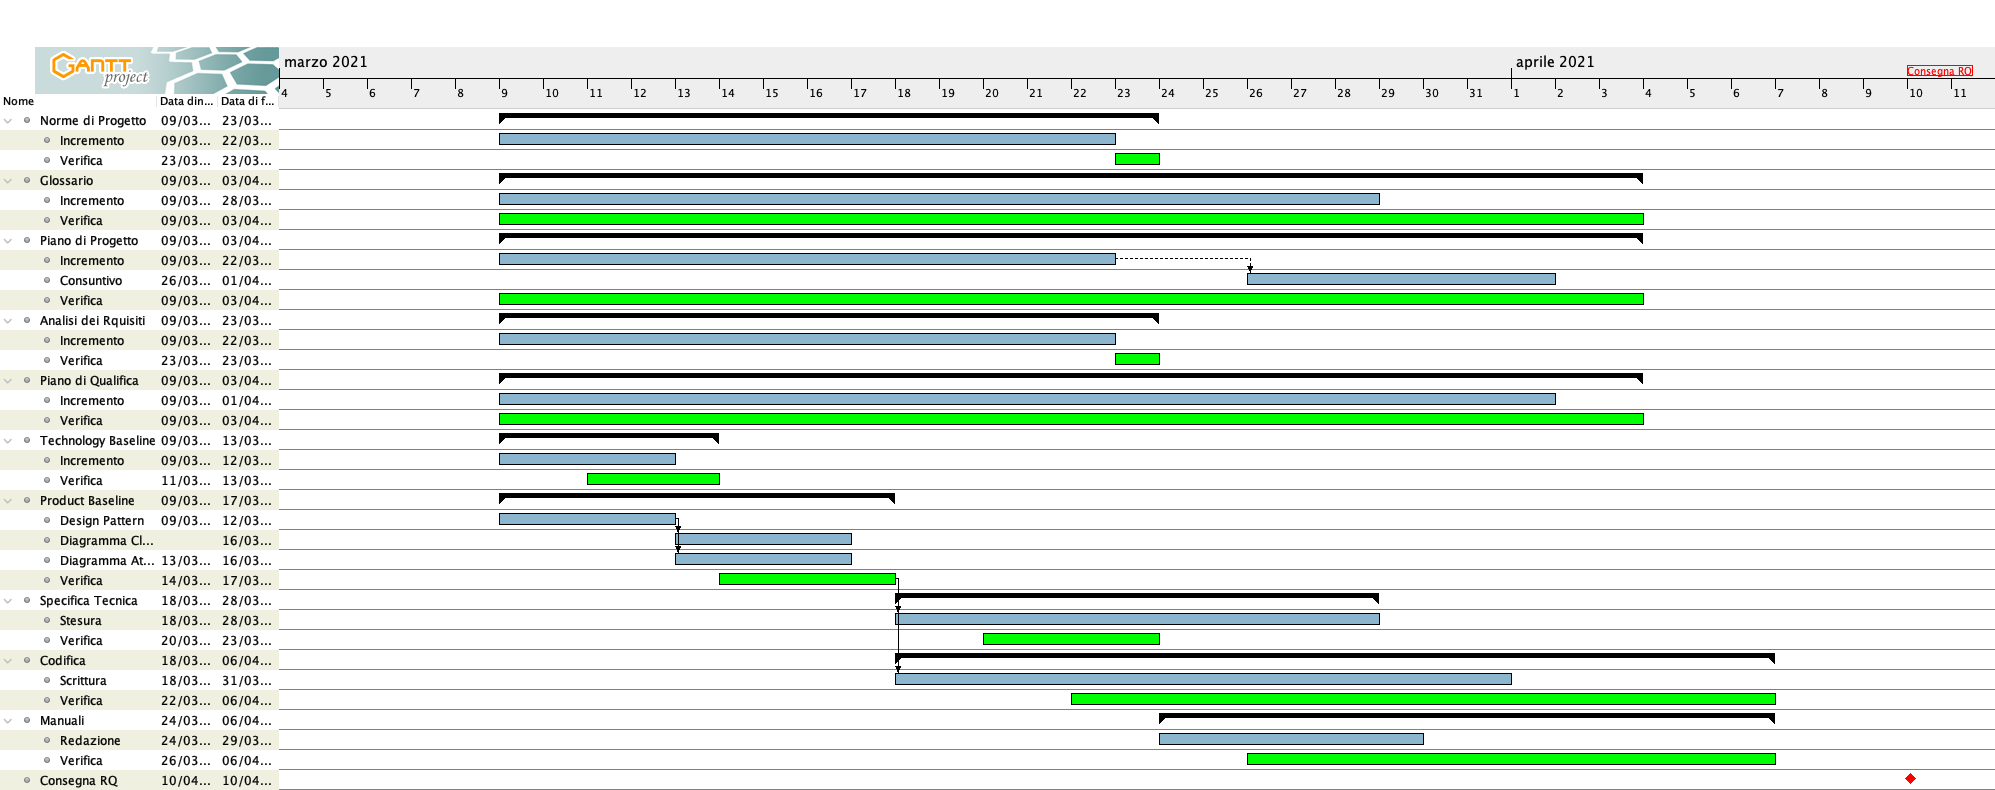
\includegraphics[width=\textwidth]{../../Immagini/GanttProgettazioneDiDettaglioECodifica}
    \caption{Diagramma di Gantt dell'avvitià di Progettazione di Dettaglio e Codifica}
\end{figure}